
\documentclass[10pt,journal]{IEEEtran}

\usepackage{mathtools}
\usepackage{algorithmic}
\usepackage{graphicx}
\usepackage{subfig}

\begin{document}
\title {Shape recognition using machine learning}
\author {\IEEEauthorblockN{Sebastian Gomez} \\
	\IEEEauthorblockA{Systems and computer engineering\\
	Universidad Tecnologica de Pereira\\
	Pereira, Colombia\\
	Email: segomez@utp.edu.co}
}
\date {July of 2010}
\IEEEpubid{978-1-4577-0286-0/11 \$26.00 \copyright 2011 IEEE}

	%\markboth{VI Congreso Colombiano de Computacion,~Vol.~6, No.~1, December 2010}
	%{Sebastian Gomez: Shape recognition using machine learning}

	\maketitle

	\begin{abstract}
		Computer vision is a growing field of computer science that intends to extract
		some useful information from images, usually taken from cameras or scanners.
		The ability to recognize shapes in images is often necessary in computer vision
		programs. 
		This article describes how to make a program able to recognize basic 
		geometrical figures by using machine learning. This article shows the image 
		processing stages until	feature extraction; Giving to the reader an idea of how
		to apply computer vision for other problems that involve shape recognition.
	\end{abstract}
	
	\begin{IEEEkeywords}
	Artificial Intelligence, Machine learning, Computer vision, Pattern Recognition
	\end{IEEEkeywords}


	\section{Introduction}
	\IEEEPARstart{W}{hen} you teach a child how to recognize basic geometrical figures such
	as a triangle, a square, or a rectangle, you do not tell the child "a square has four
	equal sides, and four 90-degree angles". Such academic language can be challenging for 
	a young and still unschooled child. You may more likely show him several examples
	of shapes and the child, after repeatedly being exposed to the different shapes, may 
	be able to learn to differentiate them on his own. \newline
	A similar approach can be used with a computer. One way of training a computer to
	recognize basic shapes is by using elements from "machine learning", an area of
	artificial intelligence. To enable a computer to differentiate basic geometrical 
	figures is not a simple task. However, this is possible by using computer vision 
	techniques. In this article, we will illustrate how to achieve computer shape 
	recognition. More specifically, our goal is to show how to design a program using
	the OpenCV library to recognize geometrical figures drawn by hand, constraining
	the paper to be white and the pencil to be black. The field of computer vision
	usually	propose 3 stages for image recognition.
	
	\section{Image filtering}
	The first stage receives as input an image an outputs an image having only
	what we need. In order to recognize geometrical figures, we must find the 
	contour of the shape. But before doing so we turn the image into gray scale.
	As any signal acquisition, the input has noise and we must filter it; To do
	so we used a Gaussian filter. We could define now the filtered gray-scale image
	as a function $I_1(x,y)$, that represents the value of the pixel located at
	$(x,y)$ as an integer between 0 and 255; Where 0 is black, 255 is white and
	all other values are some kind of gray.\newline
	As we are interested in finding the contour of the shape, we first binarize
	the image. That binarization is achieved by choosing a value T, such that any
	value above it is taken to 255, and any value below it is taken to 0.
	To choose T as a constant value is not a good idea, since it will make the
	system too dependent on light conditions. We used an approach called
	adaptive threshold, that choose the value of T for each pixel by averaging
	its neighbors. If $I_2(x,y)$ represents the binarized image and $\mu(x,y)$
	represents the mean in some area $A_2$ around $(x,y)$; We would have:
	\[ I_2(x,y) = \left\{ \begin{array}{ll}
		0   & \mbox{if $I_1(x,y) < \mu(x,y)$} \\
		255 & \mbox{otherwise}
	\end{array} \right. \]
	The computation of $\mu(x,y)$ for each $(x,y)$ in the usual way would
	be very computational expensive. A better approach for doing so was proposed by
	Shafait, Keysers and Breuel \cite{ocropus2}. They use integral images for computing
	the sum around $A_2$ in constant time for each pixel $(x,y)$; With this approach they
	can binarize the image in time $O(N^2)$ instead of the $O(N^2W^2).$ \footnote{For the
	complexity computation, they supposed that the image has size NxN pixels; And that
	the area $A_2$ around each pixel is a square of side W.}
	
	\section{Obtaining the features}
	The second stage receives as input $I_2(x,y)$, the output image of the first
	stage; and should return to us the features for the recognition stage. We used the 
	OpenCV library for all the project, this library has a function named
	\textit{cvFindContours} to find the contour of a shape once the image is
	binarized. The contour is a sequence of $(x,y)$ points at the border of an image,
	that we are going to approximate with polygon using the function 
	\textit{cvApproxPoly} of the library\footnote {If you want to know how the 
	functions \textit{cvFindContours} and \textit{cvApproxPoly} work, please 
	refer to OpenCV	documentation (See bibliography)}. \IEEEpubidadjcol
	Now we must compute a set of features from the set of points of our 
	approximated polygon. Those features must follow the following constrains:
	\begin{itemize}
		\item[1.] Using only the chosen features it should be enough to recognize the
			different kind of shapes.
		\item[2.] There must be a fixed number of features.
	\end{itemize}
	If we choose a vector $\vec{x} \in \mathbf{R}^n$ to store the features, we will
	ensure the second constraint is satisfied; Because each feature vector would have
	exactly $n$ features.
	
	\subsection{Choosing the geometrical figures and features}
	Let $C$ be the set of the classes (geometrical figures) to differentiate. That 
	$C$ would be our goal, lets define it as:
	\[C = \{ Triangle, Square, Rectangle, Rhombus \} \]
	For that set of shapes, we found one possible vector of features $\vec{x}$ with
	$n=4$ that provides enough information to differentiate each of those shapes.
	\[\vec{x} = <a_1,a_2,a_3,a_4> \]
	Where:\newline
	$a_1$ is the number of sides of the polygon\newline
	$a_2$ is the standard deviation of the sides divided by the perimeter\newline
	$a_3$ is the standard deviation of the magnitude of the angles\newline
	$a_4$ is the magnitude of the angle closest to 180 degrees\newline
	
	As our goal is to recognize geometrical figures drawn by hand, the formal definitions
	of the geometrical figures are not enough for classification. For example, you can't expect that 
	a square drawn by hand has all its sides with the same length; But you can expect 
	that the standard deviation of those lengths should be less than in a rectangle.
	Similarly, you can't expect the all the internal angles of a rectangle are
	exactly equal among them. But the standard deviation of those angles should be
	lower than in the rhombus.\newline
	However, it was observed that the standard deviation of the length of the sides
	$\sigma_l$ increased with the size of the shape; That make sense but is
	undesirable. To avoid that, $\sigma_l$ was divided by the perimeter of the shape.
	The reason to include the magnitude of the angle closest angle to 180 degrees, is
	that some times one side of the polygon can be recognized as 2 different sides;
	But with an angle really close to 180 degrees.
	To be able to recognize between triangles the other quadrilaterals, the number of
	sides should be enough in the general case.
	
	\section{Learning and classification}
	Before being able to recognize any shape, we must learn; Learning is achieved
	through a training process.  Lets say there is function $g(\vec{x})$ that 
	return the class of the object with features $\vec{x}$. 
	Let $X$ be a set with pairs $<y_i,\vec{x_i}>$ called training set, such that
	its known that $y_i$ is the class of the object with features $\vec{x}$; That is:
	\[ \forall <y_i,\vec{x_i}> \in X , y_i=g(\vec{x_i}) \]
	We can define the system to be trained as a function $f(\vec{x},\vec{p})$,
	where $\vec{p}$ is a vector containing some parameters and $\vec{x}$ has
	the same meaning as above. Then, the objective of training is to find the
	parameters $\vec{p}$ such that the error of $f$ with the data in the training
	set is minimized. Assuming that a Boolean operator return 1 if they are true
	or 0 if false, we would have:
	\[ min_{\vec{p}} \left[ E = \sum_{i=1}^{\| X \|}  
		( y_i \not= f(\vec{x_i},\vec{p}) ) \right] \]
	To model $f$, we used a binary decision tree\cite{cart}. That is a tree with one
	condition per node. In each node the condition is evaluated and depending
	on the truth value one of the two children nodes is chosen. This process
	repeats itself until a leaf is reached, and each leaf has only one class.
	That class would be the output of $f$. We perform this operation by using the
	C++ class \textit{CvDTree} of OpenCV. The final tree produced by the program to
	recognize the different shapes is shown in Figure \ref{fig:tree}.
	\begin{figure}[htb]
	\begin{center}
	\leavevmode
	\includegraphics[width=5cm]{tree.jpg}
	\end{center}
	\caption{Classifier tree for basic shape recognition}
	\label{fig:tree}
	\end{figure}
	
	\subsection{Building the training set}
	To build the training set, several shapes of the same kind were drawn with a
	dark pen in a white	piece of paper. One picture were taken to each piece of
	paper, and the file name of the picture was set such that the first letter
	represented the kind of shape drawn in that picture. \newline
	In figure \ref{fig:training} some of the pictures taken for the training set 
	are shown. If the file name starts with R, the picture contains only rectangles
	(Figure \ref{fig:r1}). If the file name starts with T, the picture contains only triangles
	(Figure \ref{fig:t1}). If the file name starts with S, the picture contains only squares
	(Figure \ref{fig:s1}). And if the file name starts with H, the picture contains only rhombus
	(Figure \ref{fig:r1}).\newline
	All the pictures with training instances are stored in a folder named ``Training''.
	Then the training process consist on reading all the pictures stored on the Training
	folder, and for each picture, all contours are extracted. Then the features are
	computed for each contour and the feature vector is added to the training set with
	the corresponding label $y_i$. Remember that the label $y_i$ is the known class of the
	input $\vec{x_i}$, and $y_i$ is known because of the file name.
		
	\begin{figure}
	\centering
		\subfloat[R1.jpg]{\label{fig:r1}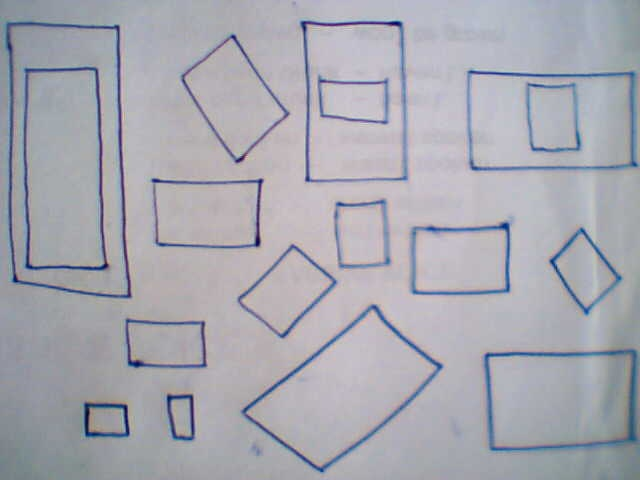
\includegraphics[height=2cm]{R1.jpg}}
		\subfloat[T1.jpg]{\label{fig:t1}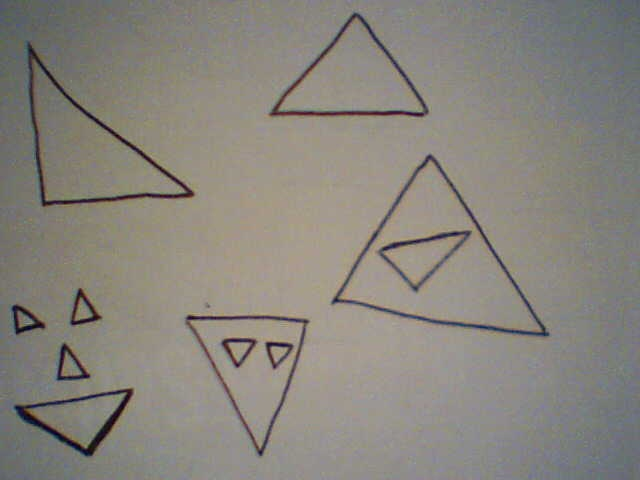
\includegraphics[height=2cm]{T1.jpg}}\\
		\subfloat[S1.jpg]{\label{fig:s1}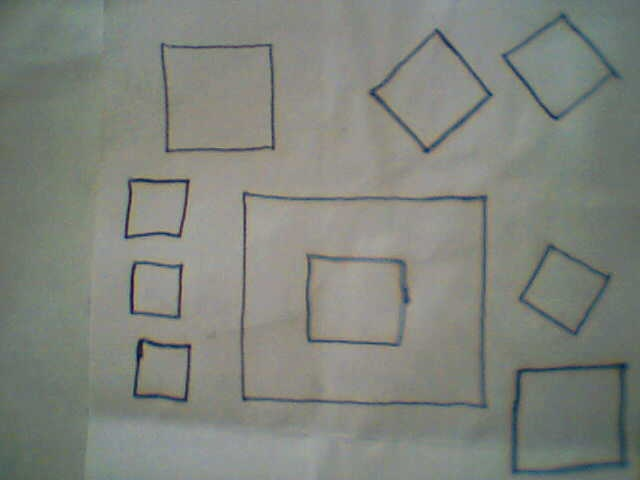
\includegraphics[height=2cm]{S1.jpg}}
		\subfloat[H1.jpg]{\label{fig:h1}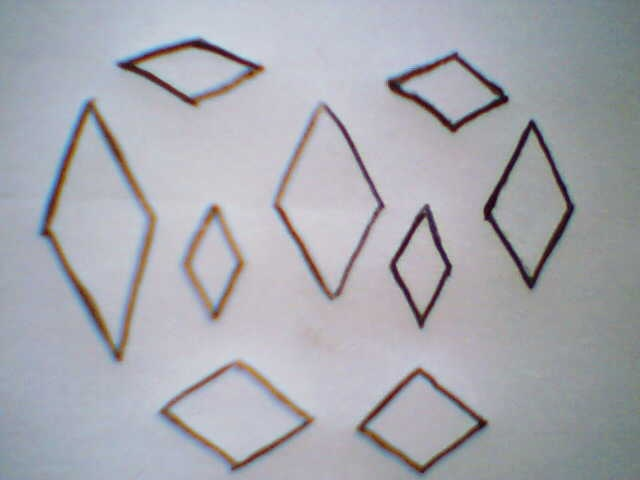
\includegraphics[height=2cm]{H1.jpg}}
	\caption{Examples of shapes in the training set}
	\label{fig:training}
	\end{figure}
	
	\subsection{Validation set}
	To test the generalization capability of the learning algorithm, it must be
	tested over a set of instances not seen during training. This set of instances is
	called validation set. The instances on the validation set should be labeled, so when
	the trained algorithm is tested with an instance on the validation set it can be known if
	the output is right or wrong.\newline
	One way of building a validation set is by removing some instances of the training set
	and adding them to the validation set. An instance was left in the training set with a
	probability of 70\% or moved to the validation set with a probability of 30\%.
	
	\section{Results and Conclusions}
	The results of the image processing stage can be seen in figure \ref{fig:transform}. The
	figure \ref{fig:org} shows an image of a rectangle as it is taken from the camera. The 
	figure \ref{fig:bin} shows the image after being transformed to gray-scale, filtered and 
	binarized using	the threshold method explained above. The figure \ref{fig:shp} shows the
	polygon that approximates the shape in figure \ref{fig:bin} with an allowed error of 10
	pixels.\newline
	After the binary decision tree was trained, it was proved against the validation set,
	the results can be seen in Table \ref{tb:result}. The table shows how many instances
	of each class are well classified (TP: True positives, TN: True negative) or
	misclassified (FP: False positive, FN: False negative).
	Only one of the shapes of the validation set
	was not correctly recognized, which means an accuracy of 97.3\%. The accuracy can
	be improved even more adding more features and more training instances. 
	Note that in this case, the trained tree (Fig \ref{fig:tree}) doesn't care about the 
	deviation of the angles for the classification of the 4 kind of shapes.\newline
	The training set consisted on 9 rhombus, 26 squares, 18 rectangles and 33 triangles. Note
	that the training set didn't have to be very big to achieve a good classification performance.
	The binary decision tree model is almost ideal to solve this problem. For
	more complex problems such as optical character recognition or face recognition,
	complex models such as neural networks or support vector should be used instead.
	
	\begin{figure}
	\centering
		\subfloat[Original]{\label{fig:org}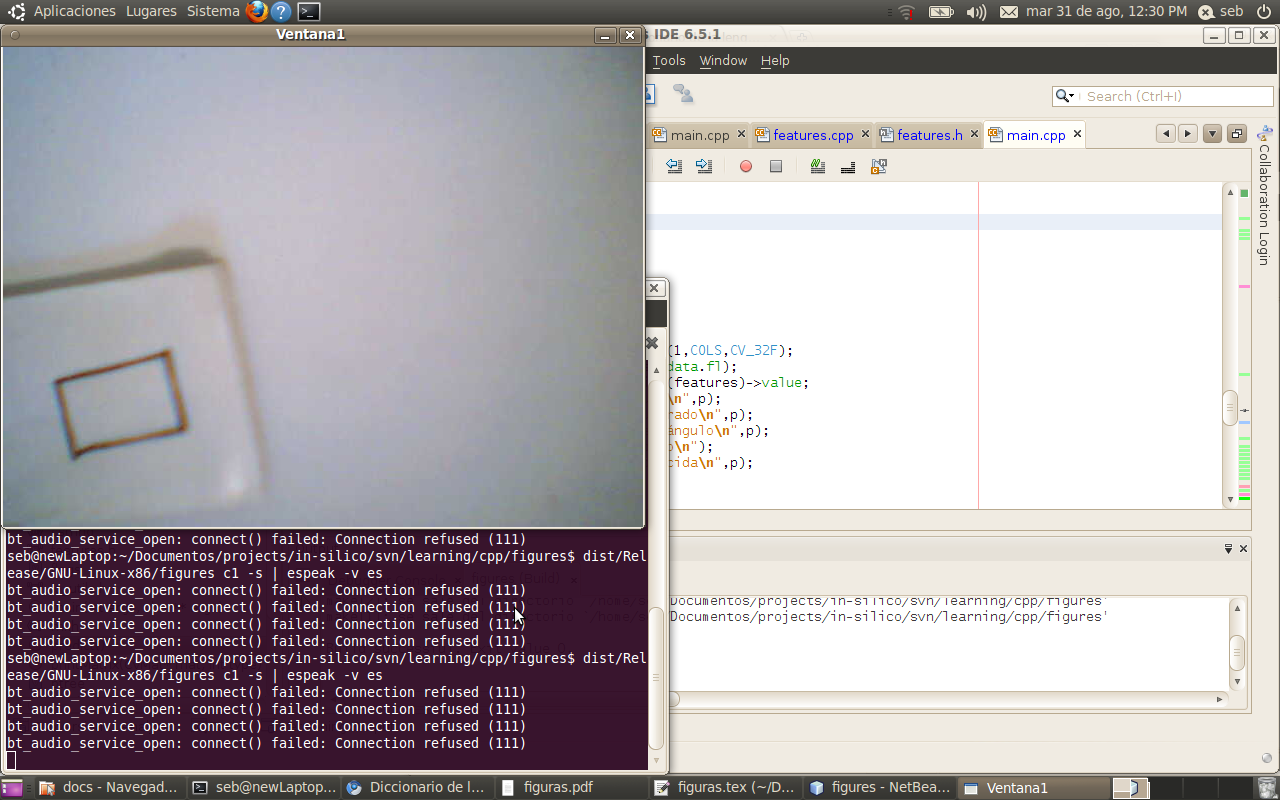
\includegraphics[height=2cm]{img1}}
		\subfloat[Binarized]{\label{fig:bin}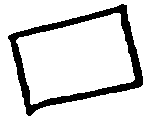
\includegraphics[height=2cm]{img2}}
		\subfloat[Polygon Approximation]{\label{fig:shp}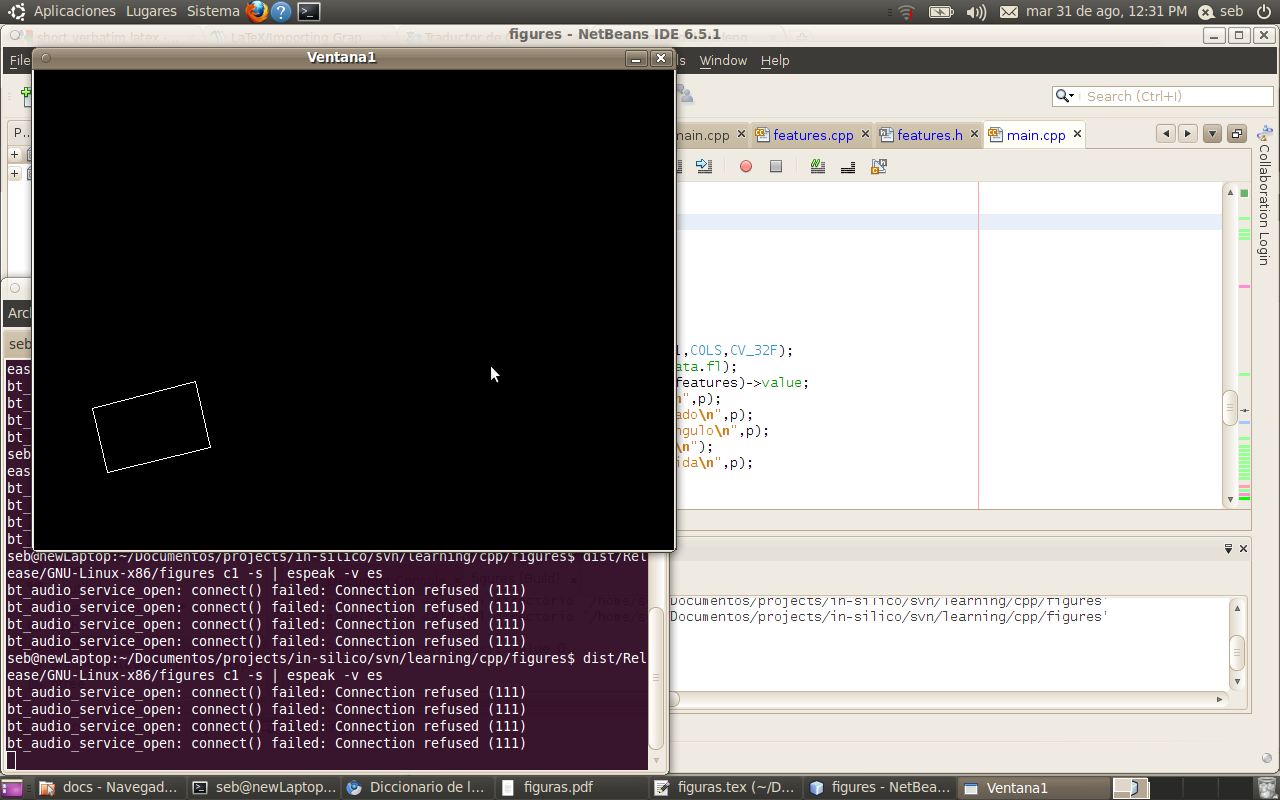
\includegraphics[height=2cm]{img3}}
	\caption{Original image and its transformations}
	\label{fig:transform}
	\end{figure}
	
	\begin{table}
	\begin{center}
	\begin{tabular}{|c|c|c|c|c|}
		\hline
		Shape & TP & TN & FP & FN \\			
		\hline
		Rhombus & 2 & 35 & 0 & 0 \\
		Rectangle & 10 & 26 & 1 & 0 \\
		Square & 11 & 26 & 0 & 0 \\
		Triangle & 13 & 23 & 0 & 1 \\
		\hline
	\end{tabular}
	\end{center}
	\caption{Accuracy of the classifier algorithm in the first experiment}	
	\label{tb:result}
	\end{table}
	
	
	
	\begin{thebibliography}{9}
	
		\bibitem{Bradski08}
			Gary Bradsi, Adrian Kaehler,
			\emph{Learning OpenCV: Computer vision with the OpenCV Library}.
			O'REILLY,
			First edition,
			2008.
			
		\bibitem{Alpaydin04}
			Ethem Alpaydin,
			\emph{Introduction to machine learning}.
			The MIT press,
			2004.
		
		\bibitem{OpenCV10}
			"The OpenCV reference",
			http://opencv.willowgarage.com/wiki/,
			2010.
			
		\bibitem{Cpp2010}
			"The C++ Resources Network",
			http://www.cplusplus.com/,
			2010.
			
		\bibitem{ocropus2}
			SHAFAITA Faisal; KEYSERSA, Daniel y BREUEL, Thomas. 
			\emph{Efficient Implementation of Local Adaptive Thresholding Techniques Using Integral Images.}
			DOCUMENT RECOGNITION AND RETRIEVAL. 
			February of 2008.
			
		\bibitem{cart}
			Breiman, L. and Friedman, J. and Olshen, R. and Stone, C. and Steinberg, D. and Colla, P.
			\emph{CART: Classification and regression trees},
			Wadsworth: Belmont, CA,
			1983.
	\end{thebibliography}
	
\end{document}
